\section{Verrattavat ohjelmointikielet}

\hl{Olisiko hyvä, jos jokaisen luvun alussa olisi pieni kuvaus luvun
sisällöstä? Tässä voisi olla tyyliin ''Tässä luvussa kuvaillaan yleisiä
ominaisuuksia verrattavista ohjelmointikielistä ja käydään läpi kunkin kielen
yksittäisiä piirteitä, ja pohditaan syitä, miksei mikään näistä ole
syrjäyttänyt C:tä''}

\hl{8. Luku 3 on myös hieman hankala lukea. Tuossa näyttäisi olevan ajatuksena
tuoda näkyviin luvun 2 alun ''parempi kuin C'' -kriteerien mukaisia asioita, mikä
on sinänsä OK. Tämäkin luku vaatii tosiaan ymmärrettävän rakenteen ja
perustelun lukijalle, mitä asioita vertailtavista kielistä kerrotaan (ja
miksi).}

\subsection{Yleisiä vertailtavien ohjelmointikielten ominaisuuksia}

C:hen vertailtavissa ohjelmointikielissä on yleisesti useita ominaisuuksia,
jotka vaikuttavat ohjelmien ajoaikaiseen nopeuteen hidastavasti, lisäävät
muistinkäyttöä tai vähentävät alustariippumattomuutta.

Yleisin näistä on automaattinen muistinhallinta, joka lisää ''roskien
keräämisen''\defword{garbage collection, GC}, jonka ajaksi ohjelman suoritus
pysäytetään. Lisäksi roskien keräämiseen perustuva automaattinen
muistinhallinta lisää muistinkäyttöä, sillä ohjelmointikieli joutuu
ajoaikaisesti seuraamaan käytössä olevia muistiosoitteita.

Monissa vertailtavissa kielissä on käytössä nimiruntelu\defword{name mangling},
joka mahdollistaa useat näennäisesti samannimiset funktiot. Tämä kuitenkin
aiheuttaa ohjelmointikielten välille yhteensopivuusongelmia, sillä toisesta
kielestä kutsuttaessa pitää tietää kutsuttavan funktion todellinen nimi.

Ohjelmointikielen ominaisuudet vaikuttavat siihen, minkälaisia
ohjelmistoarkkitehtuureja kielellä tehdään\citationneeded. Moderneissa
ohjelmointkielissä virheiden käsittely on yleensä toteutettu kahdella tavalla:
toinen on poikkeavat paluuarvot ja toinen on poikkeuksien heittäminen.
Yleisesti ottaen kaikki ohjelmointikielet tukevat ensimmäistä ja suurin osa
toista tapaa. Poikkeusten käsittely on hieman hitaampaa ja aiheuttaa hieman
suuremman muistinkäytön, ja tehokkaaseen ohjelmakoodiin pyrkiessä yleensä
vältetään poikkeusten käyttämistä\citationneeded. Monet poikkeuksia tukevien
ohjelmointikielten vakiokirjastot kuitenkin pakottavat hallitsemaan
virhetilanteita poikkeuksilla.

\subsection{Ada}

Ada on Yhdysvaltain puolustusministeriön kehittämä ohjelmointikieli, joka
suunniteltiin korvaamaan kaikki muut puolustusministeriön käyttämät
ohjelmointikielet~\citep{adahistory}. Ada on hyvin moneen taipuva kieli, sillä
se on suunniteltu hallitsemaan monia eri käyttötarkoituksia matalan tason
bittitason ohjelmoinnista korkean tason arkkitehtuureihin.

Ohjelmoinnin tehostamiseksi Adassa on sekä poikkeukset että automaattinen
muistinhallinta. Nämä kuitenkin hidastavat kieltä hieman aikaisemmin todetuistä
syistä. Lisäksi C-kielen kanssa yhteensopivuus on kielen taipuvuudesta johtuen
hankalaa -- jokainen kutsuttava C-funktio on yksitellen määritettävä
kutsukonvention\defword{calling convention} kanssa~\citep[s.~471]{ADA12}. Adan
alustariippumaton C-tuki on kuitenkin äärimmäisen kattava, paikoitellen C:n
omaa tukea kattavampi (C:n standardi ei kuvaile esimerkiksi kutsukonventioita,
vaan ne on jätetty kääntäjäspesifeiksi asetuksiksi).

\subsection{C++}

C++ on Bjarne Stroustrupin 1980-luvusta eteenpäin kehittämä kieli, jonka
yhtenä tarkoituksena on yhdistää Simula-kielen ominaisuudet ohjelman
organisointiin yhteen C:n tehokkuuden ja joustavuuden
kanssa~\citep{cpphistory}. C++ on nykypäivänä suosittu tehokkuutensa ja
monipuolisuutensa takia monimutkaisissa ohjelmistoissa, kuten
palvelinohjelmistoissa, kuvankäsittelyohjelmistoissa sekä
peleissä~\citep{cppapps}.

C++ on kehitetty C:n pohjalta, ja siinä onkin erittäin hyvä C-tuki. Koska
C++\hyp{}funktiot nimirunnellaan eikä nimiruntelua ole määritelty tarkasti C++:n
standardissa, C++-koodia on hankalaa kutsua jopa samalla alustalla eri
C++-kääntäjien välillä. C-koodin otsikkotiedostoissa\defword{header file} on
usein alussa C++-koodia, joka laittaa nimiruntelun pois päältä. Näin
C++-ohjelmat voivat helposti kutsua C-ohjelmien kirjastokutsuja -- C++-ohjelmat
voivat usein käyttää C-kielen otsikkotiedostoja ilman muita muokkauksia.

Virheidenkääsittely on toteutettu poikkeuksilla, jotka aiheuttavat pienen
hidastuksen. C++:ssa on myös käytettävissä viitemäärälaskettu\defword{reference
counting} muistinhallinta (vakiokirjaston \texttt{std::shared\_ptr}), jolla
voidaan käyttää ajoaikaisesti varattua muistia ilman muistivuotoja. C++:ssa ei
ole roskien keräystä, vaan kun viimeinen viite olioon poistetaan, myös varattu
muisti vapautetaan. Tällöin ohjelman suorituksen aikana ei tule
roskienkeräystaukoja.

C++-ohjelmat rakennetaan usein C++:n luokkien ympärille, jotka usein sisältävät
malliohjelmointia\defword{template programming}. C++:n toteutuksessa jokaisesta
erillisestä mallin instanssista luodaan lopulliseen ohjelmaan kopio
funktioista, joka kasvattaa ohjelmien kokoa. Tämä on tehty, jotta kääntäjät
voisivat optimoida jokaisen luokan instanssin erikseen. Tämä kuitenkin usein
kasvattaa sekä kääntämisaikoja että ohjelmien kokoa.

\subsection{D}

D on 2000-luvun alussa Digital Mars -yrityksen julkaisema ohjelmointikieli,
jonka tarkoituksena on mahdollistaa helposti tehokkaan ohjelmakoodin
kirjoittaminen helposti ja turvallisesti~\citep{dhistory}. Vaikka D-kielessä on
olemassa automaattinen muistinhallinta, D:n \emph{BetterC}-tila tekee kielestä
''paremman C:n'' poistamalla ajoaikaiset ominaisuudet, mukaan lukien
automaattisen muistinhallinnan~\citep{dbetterc}. Tällöin kielestä poistuu
useita ominaisuuksia, mutta esimerkiksi D:n käännösaikaista makrojärjestelmää
voi käyttää.

C-koodin kutsuminen on melko helppoa, mutta ei aivan saumatonta, sillä jokainen
kutsuttava funktio tulee määritellä erikseen -- D ei ymmärrä C:n
otsikkotiedostoja. Tämä kuitenkin onnistuu yhdellä rivillä jokaista C:n
funktiota kohden, sillä D:n tyyppijärjestelmä on hyvin lähellä C:tä. D:lle on
myös olemassa useita työkaluja otsikkotiedostojen automaattiseen muuntamiseen,
kuten \texttt{htod}-työkalu~\citep{htod}. Työkalut eivät kuitenkaan ole
täydellisiä, sillä useiden D:n ominaisuuksien semantiikka ei ole C:n kanssa
yhteensopiva.

\subsection{Go}

\hl{Taivutus; Go:ssa, Gossa, Go-kielessä, Golangissa...? Ainakin se lautapeli
taivutetaan toisen mukaan, mutta käytin nyt kolmatta muotoa, koska Wikipedia
näyttäisi suosivan sitä.}

Go on Googlen 2000-luvun loppupuolella kehittämä ohjelmointikieli, jonka
tarkoituksena on yhdistää kääntöaikaisesti tyypitetyn ohjelmointikielen
turvallisuus ja tehokkuus ajoaikaisesti tyypitettyjen ohjelmointikielten
helppokäyttöisyyteen~\citep{gohistory}. Toisin kuin monissa moderneissa
C-perheen kielissä, Go-kielessä ei ole luokkia, vaan pelkkiä tietueita ja
rajapintoja.

Go-kielessä ei ole mahdollista kirjoittaa käännösaikaisesti tyyppitarkistettua
tyyppiparametreja käyttävää koodia, mutta ohjelmat voivat ajoaikaisesti
peilauksen\defword{reflection} kautta tutkia tietueiden rakennetta.
Tämän mahdollistaminen kasvattaa ohjelmakoodin kokoa, sillä rajapinnan mukana
on säilytettävä rajapinnan oikeaa tyyppiä. Tämä kuitenkin yksinkertaistaa
ohjelmien kirjoittamista, sillä ohjelmoijan ei tarvitse miettiä
kirjoittamishetkellä monimutkaisia tyyppejä~\citep[esim.][kalvo 8]{gohistory}.

Go-kielen virheidenkäsittely on toteutettu useissa kohdissa C:n tavoin;
funktioista palautetaan virheellisissä tilanteissa virheellinen arvo. Tämä
tosin tehdään usein palauttamalla erillinen \texttt{Error}-tyyppiä oleva arvo
-- Go mahdollistaa useamman kuin yhden paluuarvon. Go-kielessä on myös
poikkeukset, joita suositellaan käyttävän vain poikkeuksellisissa
tilanteissa~\citep{effectivego}.

C:n kutsuminen Go-kielestä ei ole aukotonta: koska Go on muistinkäytöltä
turvallinen kieli, erityisesti muistin jakaminen C:n ja Go-kielen välillä on
hankalaa. Lisäksi C:n funktio-osoittimia ei voi kutsua Go-kielen
puolelta~\citep{cgo}. Go mahdollistaa C-otsikkotiedostojen suoran käytön
ohjelmakoodista, mikä helpottaa C-koodin kutsumista.

\subsection{Rust}

Rust on Mozilla Foundationin kehittämä ohjelmointikieli, joka on suunniteltu
turvalliseksi, rinnakkaiseksi ja käytännölliseksi
järjestelmäohjelmointikieleksi~\citep{rustfaq}. Rustissa on monimutkainen
tyyppijärjestelmä, jolla ohjelmat voivat todistaa esimerkiksi turvallisen
rinnakkaisajon, ilman että ohjelmaan tulee ajoaikaisia rajoitteita tai
hidastuksia.

Kuten Go-kielessä, Rustissa voi myös käyttää poikkeuksia. Rustin
virheidenhallinta on muutenkin lähellä Go-kielen virhehallintaa -- Rustin
ohjekirja opastaa käyttämään mieluummin paluuarvoja kuin
poikkeuksia~\citep{rusterrorhandling}.

Rustin monimutkainen tyyppijärjestelmä kannustaa kirjoittamaan turvallisia
ohjelmia, Tietorakenteiden mutatoiminen on tehty tietoisesti hankalaksi, sillä
monimutkaisissa ohjelmissa holtittomasti muuttuva tila on usean vian syynä, ja
muuttumaton tila tekee moniajettujen ohjelmien toteutuksesta huomattavasti
helpompaa\citationneeded. Ohjelmien tilaa voi muuttaa erityisillä muuttuvilla
viitteillä\defword{mutable reference}, joita voi yleensä olla vain yksi kutakin
viitettä kohden kerrallaan.

Turvallisuudella on kuitenkin hintansa -- Rust-ohjelmat vievät enemmän tilaa
kuin vastaavat C-ohjelmat. Jos Rust-ohjelmista poistaa standardikirjaston ja
käyttää suoraan C:n standardikirjastoa, ohjelmasta saa käytännössä
samankokoisen kuin vastaavasta C-kielellä kirjoitetusta
ohjelmasta~\citep{rustbinarysize}. Samalla tosin suurin osa Rustin
ominaisuuksista jää pois. Rustin turvallisuus vaatii myös monimutkaisen
tyyppijärjestelmän, joka on vaikeampi opetella kuin yksinkertaisemman kielen
tyyppijärjestelmä.

Rust ei pysty suoraan käsittelemään C:n otsikkotiedostoja, mutta D:n tavoin
Rustille on saatavilla työkaluja otsikkotiedostojen automaattiseen
muuntamiseen~\citep{rustbindgen}. Rust kuitenkin suosittelee jokaisen kirjaston
kohdalla käsin ympäröimään C-kirjaston funktiot, sillä C:n tyyppimäärittelyt
eivät tarjoa Rustin vaatimaa tarkkuutta funktioiden turvallisuudesta.

\subsection{Yhteenveto}

Yksikään vertailtavista kielistä ei täytä kaikkia luvussa~\ref{sec:abs}
määriteltyjä rajoitteita. Yksikään kielistä ei täytä muistinkäytön rajoitteita,
jonka lisäksi saumaton yhteistyö C:n kanssa onnistuu vain C++:n
kanssa. Kaikki vertailtavat kielet tukevat vierasfunktiorajapintoja C:n
mukaisesti, eli kielet voivat kutsua muita kieliä C-rajapintojen läpi.
C++ ja Rust ovat hyvin lähellä C:tä käännettyjen ohjelmien koossa, mutta
häviävät C:lle laajojen vakiokirjastojen takia. Molemmat ovat myös hyvin
monimutkaisia kieliä. Vain C++ ja Go voivat sisällyttää ohjelmiin C:n
otsikkotiedostoja, kun taas Ada, D ja Rust vaativat jokaisen funktion
määrittämistä. 

\begin{table}[ht!]
    \begin{adjustbox}{center}
    \begin{tabular}{@{}lllll@{}} \toprule
        Kieli & Nimiruntelu   & Muistinhallinta                                     & C:n VFR               & muiden kielten VFR \\ \midrule
        Ada   & hallittavissa & automaattinen                                       & Työläs mutta kattava  & C, C++, Fortran, Cobol \\
        C++   & on            & manuaalinen                                         & Lähes saumaton        & C:n läpi \\
        D     & on            & molemmat                                            & Työläs mutta kattava  & C:n läpi \\
        Go    & on            & automaattinen                                       & Epätäydellinen        & C:n läpi \\
        Rust  & hallittavissa & manuaalinen\footnote{Borrow Checkerin hallitsemana} & Työläs mutta kattava  & C:n läpi \\ \bottomrule
    \end{tabular}
    \end{adjustbox}
    \caption{
        Kielten ominaisuuksien yhteenveto.
    }
    \label{table:properties}
\end{table}

\FloatBarrier

\newpage

Benchmarks gamen tulokset myös heijastavat näitä tuloksia -- C++ ja Rust ovat
nopeudeltaan hyvin lähellä C:tä, kun taas Ada ja Go ovat huomattavasti
hitaampia.

\FloatBarrier

\begin{figure}[ht!]
    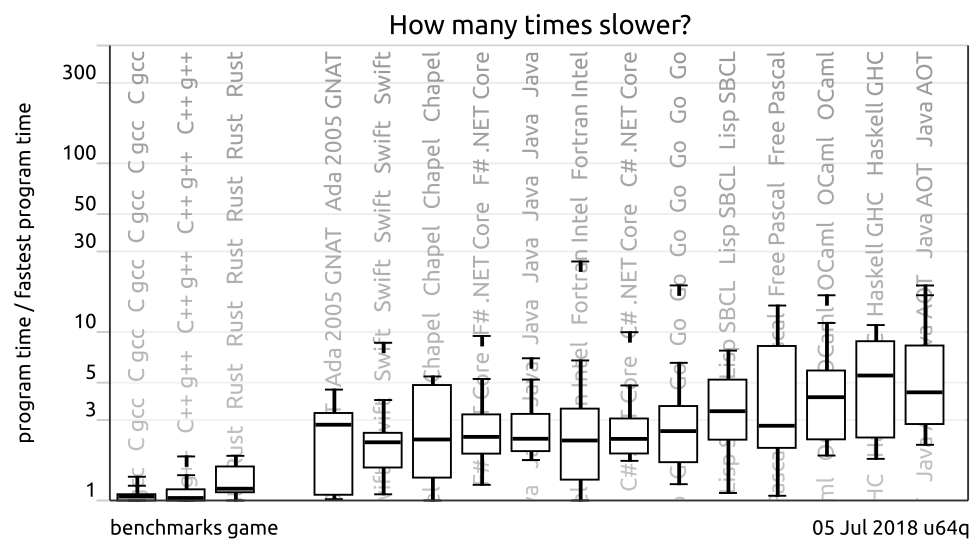
\includegraphics[width=\textwidth]{benchmarksgame.png}
    \caption{
        Benchmarks gamen~\citep{benchmarks} julkaisema kuvaaja
        ohjelmointikielten nopeuksista. C, C++ ja Rust ovat hyvin lähellä
        toistensa nopeuksia, kun taas Ada ja Go ovat selkeästi hitaampia.
        C++-versiot ovat erittäin lähellä C-versioiden nopeuksia, ja
        yksittäiset suorituskykytestit ovat nopeampia C++:lla.
    }
    \label{fig:benchmarksgame}
\end{figure}

\FloatBarrier

\hl{Tänne lisää tekstiä.}
